\chapter{数理分析}
乍一看这个“数理分析”的标题感觉怪怪的,究竟什么是数理分析?在本章的最后有介绍,这是一种重要的数学思想。

在本章中,您将学会解不等式、求代数式的最值值域以及解方程。

\section{不等式}
在初中我们仅仅学了几种不等式的解法,这些很显然是不够的。在这里我们将学习更多的,以及奇奇怪怪的不等式的解法。

\subsection[有名]{有名不等式}
为了方便起见(真的吗?),我们把一些具有明显特征的不等式的集合称为\textbf{有名不等式}。解这些有名不等式必须按照既定的规则去解,否则就不对了。

\subsubsection{一元二次不等式}
如果您去翻一翻教科书,就会发现一元二次不等式的解法好复杂\footnote{这里参照的是沪教版的教科书。}。其实教科书仅仅把可能出现的结果罗列了一遍,并没有简化解法。

那现在重新定义一元二次不等式的解法:对于$ax^2+bx+c>0$且$a>0,\Delta>0$的情况下,大于为一元二次方程的两根之外(如果$x_1<x_2$,则解集为$(-\infty,x_1)\cup(x_2,+\infty)$);小于为两根之间。

\begin{example}
	解不等式$-x^2-5x-4\geq0$
\end{example}
\begin{proof}[解]
	由于二次项系数小于$0$,先变形:\[x^2+5x+4\leq0\]

	后解其对应的方程:\[x^2+5x+4=0\Rightarrow x_1=-4,x_2=-1\]

	转换为不等式的解集:\[x\in[-4,-1]\qedhere\]
\end{proof}

$\Delta\leq0$的情况太麻烦了,我们可以选择画出不等式对应二次函数的图像后再给出解集(无非就是一个解、$\mathbb{R}$或$\emptyset$)。

\subsubsection{分式不等式}
在初中我们也学习了分式方程的解法,千万不要和解分式不等式搞混了。

分式不等式的解法如下:

\begin{enumlist}
	\item 先移项、通分、化标,变为$\frac{x-a}{x-b}\gtrless0$
	\item 可将其看成解$(x-a)(x-b)\gtrless0$的问题
\end{enumlist}

若符号为$\leq$或$\geq$,将分母对应的根由闭变为开。

\subsubsection{绝对值不等式}

\subsubsection{最简指对不等式}
本小节介绍的是\textbf{最简}指对不等式的解法,即解它们的标准形式:\[a^x\gtrless b\text{和}\log_ax\gtrless b\]

\subsection[本质]{用本质解不等式}
在上一小节中我们学习了一些具有明显特征的不等式的解法,这仅仅是一半。接下来我们要面对的是一些奇奇怪怪的不等式。

\section{值域}
顾名思义,值域就是函数因变量(即$y$)的取值范围。

\subsection[本质]{本质(有图)}
一个函数有图像,画图然后在图上看出值域就行了:

\begin{enumlist}
\item 作图
\item 描深定义域
\item 根据定义域由下往上找到值域的范围
\end{enumlist}

在第\ref{sec:mathsAnalysis-derivative-studyPorpertyOfFunction-figureOfFunction}节中,我们会了解到导数也可以用来求任何函数的值域。

\begin{example}
	求$y=x^2-2x, x\in(0,3)$的值域
\end{example}
\begin{proof}[解]
	先作如图\ref{fig:figure-of-a-function-and-its-domain}的函数图像\footnote{把求值域过程中的函数图像画出来就非常不好看,我们只画这一次。},描深定义域。

	\begin{figure}[htbp]
		\centering
		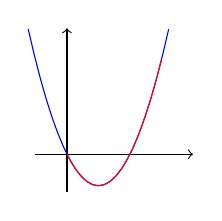
\begin{tikzpicture}[scale=0.4]
			\draw[->] (-1, 0) -- (4, 0);
			\draw[->] (0, -1.2) -- (0, 4);
			\draw[blue, domain=-1.23:3.23] plot(\x, \x * \x - 2 * \x);
			\draw[red, domain=0:3] plot(\x, \x * \x - 2 * \x);
		\end{tikzpicture}
		\caption{画图、描深}
		\label{fig:figure-of-a-function-and-its-domain}
	\end{figure}

	可得其最低点纵坐标为$-1$(是函数的顶点),两端点的纵坐标分别为$0$和$3$,故该函数值域为$[-1,3)$。
\end{proof}

\subsection[复合]{复合(无图)}
但是有些函数的图像你可是画不出来的,比如$y=4^x-2^{x+1}+1$。那就应该使用复合函数求值域的方法了。

如果一个函数$y=f(x)$可复合成$t=g(x)$和$y=f(t)$,那么可先求$g(x)$的值域,记为$A$。然后以$A$为定义域求$f(t)$的值域
(其中$f$、$g$均可作图)。

\subsubsection{根式复合}
\subsubsection{分式复合}

\subsection{非复合}
上面介绍了这么多的复合函数求值域的方法,虽然多,但不可能用在所有函数上。那这些无法复合函数我们就不能求出它们的值域。

但是我们非常的幸运,拿到了一个单调函数(或者说函数在定义域内单调),那还是有办法的,直接代端点就可以了。

\begin{example}
	求$y=(\frac{1}{2})^x+(\frac{1}{3})^x,x\in(-\infty,2]$的值域
\end{example}
\begin{proof}[解]
	由题意得,函数单调递减。

	$\therefore y\in[\frac{13}{36},+\infty)$
\end{proof}

\section{何为数理分析}
在前面的小节中,我们学会了求解三样东西:不等式、值域和方程。它们是数理分析的主要手段。

数理分析的基本思想:等式(即方程)用掉一个等式,可以减少一个未知数的个数(即消元),最终获得只含一个未知数的等式、代数式或不等式。

所谓的数理分析即:在正式计算前的一种预测,即将多于等式的未知数全部用掉后,在最终一个等式的情况下,未知数还剩几个:

\begin{desclist}
	\item[若只剩一个未知数] 可求值
	\item[若剩两个未知数] 则可求范围
	\item[若剩超过两个未知数] 则此题还有变数(可能是条件还没有找到,可能需要等待一个巧合,可能是双变量等等)
\end{desclist}
\[\begin{aligned}
	\begin{cases}
		f(x,y,z)=0 \\
		g(x,y,z)=0 \\
		h(x,y,z)=0
	\end{cases}&\text{可分别解得$x,y,z$}
	&\begin{cases}
		f(x,y,z)=0 \\
		g(x,y,z)=0
	\end{cases}&\text{可求$x,y,z$的范围} \\
	\begin{cases}
		f(a,b,c,d)=0 \\
		g(a,b,c,d)=0
	\end{cases}&\text{未必可解}
	&\begin{cases}
		f(x)>0 \\
		g(x)>0
	\end{cases}&\text{分别解完后求交集} \\
	\begin{cases}
		f(x,y)>0 \\
		g(x,y)>0
	\end{cases}&\text{线性规划(同向可加)}
	&\begin{cases}
		f(x,y)>0 \\
		g(x,y)=0
	\end{cases}&\text{利用$g$消元,可解$f$}
\end{aligned}\]

注意可解不等式只能含一个变量,不等式组也只能含一个变量,不等式组只是解集的交并关系,不等式不可用来消元。

多变量不等式是线性规划问题(同向可加性是最简线性规划问题)。

在有多个字母的情况下(尤其是涉及到复数),使用数理分析可快速的找到解题思路。
